%------------------------------------------------
%	PACKAGES AND THEMES
%------------------------------------------------

% this is a 4:3 layout.
\documentclass{beamer}
% for 16:9 use this command:
% \documentclass[aspectratio=169]{beamer}

\mode<presentation> {
\usetheme{metropolis}
\setbeamertemplate{caption}[numbered]
\setbeamertemplate{navigation symbols}{} % hide navigation symbols
}

\usepackage{graphicx} % images
\usepackage{algorithm2e}
\usepackage{mathtools}
\DeclarePairedDelimiter{\ceil}{\lceil}{\rceil}
\usepackage{algpseudocode}
\usepackage{booktabs} % allows the use of \toprule, \midrule and \bottomrule in tables
\usepackage[ngerman]{babel}
\usepackage[utf8]{inputenc}
\usepackage[T1]{fontenc}
\usepackage{mathtools}
\usepackage{xcolor}
\usepackage{listings} % code
\usepackage{pgf,tikz} % drawing
\usepackage{pifont} % new symbols
\usepackage{hyperref} % pretty links
% \usepackage{algorithmicx}
% \usepackage{algpseudocode}
% \usepackage[linesnumbered,ruled]{algorithm2e}

\usepackage{lmodern}
\usepackage{subcaption}
\usepackage{textcomp}
% \usepackage{array}
% \usepackage{longtable}
% \usepackage{verbatim}
%\usepackage{tabularx}
\captionsetup[figure]{font=footnotesize}

\usepackage{amsmath}
\usepackage{amssymb}
\usepackage{amsthm}
% \usepackage{comment}
% \usepackage{enumitem}
% \usepackage[binary-units=true]{siunitx}
% \usepackage{thmtools}
\usepackage{csquotes}
\usepackage{tikz}
\usepackage{float}
\usetikzlibrary{automata,positioning}

% color settings for links
\hypersetup{
    colorlinks=true,
    urlcolor=blue,
    linkcolor=black,
    citecolor=green!50!black
}

\definecolor{mygreen}{RGB}{1,135,1}

\newcommand{\cmark}{\ding{51}}  % checkmark
\newcommand{\xmark}{\ding{55}}  % xmark
\newcommand\scalemath[2]{\scalebox{#1}{\mbox{\ensuremath{\displaystyle #2}}}}

% \useoutertheme{miniframes} % navigation design
\useinnertheme{circles} % use non shiny circles (itemize, etc.)

% Main slide colors
% dunkel, hell, mittel
% \definecolor{pale}{RGB}{232, 236, 237}
% \definecolor{prim}{RGB}{53, 109, 120}
% \definecolor{sec}{RGB}{104, 170, 183}
% \definecolor{tert}{RGB}{109, 155, 168}
% \definecolor{quat}{RGB}{9, 59, 68}

\definecolor{pale}{RGB}{232, 236, 237}
% \definecolor{prim}{RGB}{153, 194, 173}
% good: \definecolor{prim}{RGB}{27, 33, 42}
\definecolor{prim}{RGB}{32, 43, 50}
\definecolor{sec}{RGB}{217, 232, 224}
\definecolor{tert}{RGB}{0, 82, 41}
% save
\definecolor{quat}{RGB}{0, 82, 41}

\setbeamercolor{palette primary}{bg=prim,fg=pale}
\setbeamercolor{palette secondary}{bg=sec,fg=pale}
\setbeamercolor{palette tertiary}{bg=tert,fg=pale}
\setbeamercolor{palette quaternary}{bg=quat,fg=pale}
\setbeamercolor{structure}{fg=prim} % itemize, enumerate, etc
\setbeamercolor{section in toc}{fg=prim} % TOC sections

% Block colors
\definecolor{example_color}{RGB}{93, 137, 98}
\definecolor{alert_color}{RGB}{175, 79, 72}

\setbeamercolor{normal text}{fg=prim!20!black,bg=pale!25!white}
\setbeamercolor{alerted text}{fg=alert_color!25!black}
\setbeamercolor{example text}{fg=example_color!25!black}

\setbeamercolor{block title example}{fg=white,bg=example_color}
\setbeamercolor{block body example}{fg=black,bg=example_color!10!white}
\setbeamercolor{block title alerted}{fg=white,bg=alert_color}
\setbeamercolor{block body alerted}{fg=black,bg=alert_color!10!white}

% Override palette coloring
\setbeamercolor{subsection in head/foot}{bg=quat,fg=pale}

\setbeamertemplate{frametitle}{%
    \nointerlineskip%

    \begin{beamercolorbox}[wd=\paperwidth,ht=2.5ex,dp=1ex]{frametitle}
        \hspace*{1ex}\insertframetitle%
        \ifx\insertframesubtitle@empty\else%
        {~\tiny\textcolor{quat!35!black}{\insertframesubtitle}}%
        \fi%
    \end{beamercolorbox}%
}

% math-command for bigger norm
\newcommand\norm[1]{\left\lVert#1\right\rVert}

% use this to include other files
% in this case style definitions for code
% alternative: \include{dateiname}
\lstdefinestyle{latex}{
    language=[LaTeX]TeX,
    inputencoding=utf8,
    basicstyle=\ttfamily,
    keywordstyle=\color{blue!60!black}, % use 60 percent blue and 40 black
    commentstyle=\color{cyan!60!black},
    tabsize=2,
    emph={document,itemize,enumerate,center,tabular,table,
    figure,wrapfigure,minipage,columns,align,bmatrix,
    lstlisting,beamer,frame,tikzpicture},
    emphstyle=\color{magenta!60!black},
    morekeywords={lstset,includegraphics,theenumi,labelitemi,column,color,url,href}
}

\lstdefinestyle{inline_latex}{
    language=[LaTeX]TeX,
    inputencoding=utf8,
    basicstyle=\ttfamily,
    resetmargins= true,
    belowcaptionskip=0pt,
    aboveskip=0pt,
    belowskip=0pt,
    keywordstyle=\color{blue!60!black},
    commentstyle=\color{cyan!60!black},
    emph={document,itemize,enumerate,center,tabular,table,
    figure,wrapfigure,minipage,columns,align,bmatrix,
    lstlisting,beamer,frame,tikzpicture,Parameter},
    emphstyle=\color{magenta!60!black},
    morekeywords={lstset,includegraphics,theenumi,labelitemi,column,color,url,href,Befehlsname}
}

\lstdefinestyle{cpp}{
    language=C++,
    basicstyle=\ttfamily,
    keywordstyle=\color{blue!90!black},
    stringstyle=\color{magenta!60!black},
    commentstyle=\color{green!35!black},
    morecomment=[l][\color{gray!60!black}]{\#},
    tabsize=2
}

\lstdefinestyle{empty}{
    basicstyle=\rmfamily,
    keywordstyle=\bfseries,
    commentstyle=\color{black}\itshape
}

\lstset{style=latex}

%------------------------------------------------
%	TITLE PAGE
%------------------------------------------------

\selectlanguage{ngerman}
\title[]{Mobility-Traffic Correlations}

\author{Tim Bohne}
\institute[]
{
\textit{Bachelor-Seminar: Mobility and Traffic in Computer Networks}
\medskip
}
\date{\today}

% make slide at the beginnig of each section
\AtBeginSection[]{
{\setbeamercolor{background canvas}{bg=white}}}

% where images are locatied
\graphicspath{{./images/}}

\begin{document}

\begin{frame}[plain] % plain slides dont have navigation bars etc.
\titlepage % Print the title page as the first slide
\end{frame}

\begin{frame}
\frametitle{Übersicht} % table of contents slide
\tableofcontents
\end{frame}

%------------------------------------------------
\section{Motivation}
%------------------------------------------------

\begin{frame}
\frametitle{Motivation}
\textit{\textquote{Analyzing Mobility-Traffic Correlations in Large WLAN Traces: Flutes vs. Cellos}}
\newline\newline\newline
\textbf{Isolierte Betrachtung}\newline
Aktuelle Modelle erfassen nicht das Zusammenspiel von Mobilität und Datenverkehr\newline\newline
\textbf{Veraltete Daten}\newline
Trace-basierte Modelle verwenden i.d.R. Datensätze aus der Prä-Smartphone-Ära
\begin{figure}
\centering
\end{figure}
\end{frame}

\begin{frame}
  \frametitle{Fragestellungen}
  \begin{itemize}
    \item Wie unterscheiden sich Mobilitäts- und Datenverkehr- Charakteristiken zwischen den unterschiedlichen Gerätetypen,
    Zeiten und Orten?\newline
    \item Wie stehen diese Charakteristiken zueinander in Beziehung?\newline
    \item Sollten neue Modelle entwickelt werden, die diese Unterschiede berücksichtigen?
\end{itemize}
\end{frame}

\begin{frame}
  \frametitle{Intuitive Beispiele}
  \begin{figure}
    \centering
    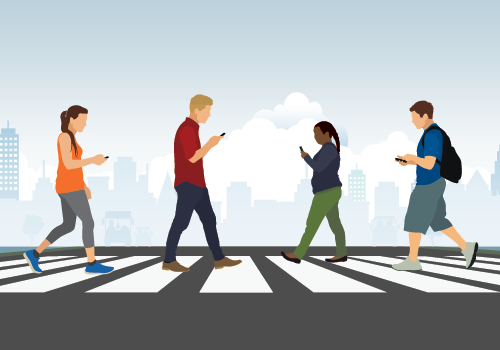
\includegraphics[width=0.55\textwidth]{images/smartphone_walking.png}
    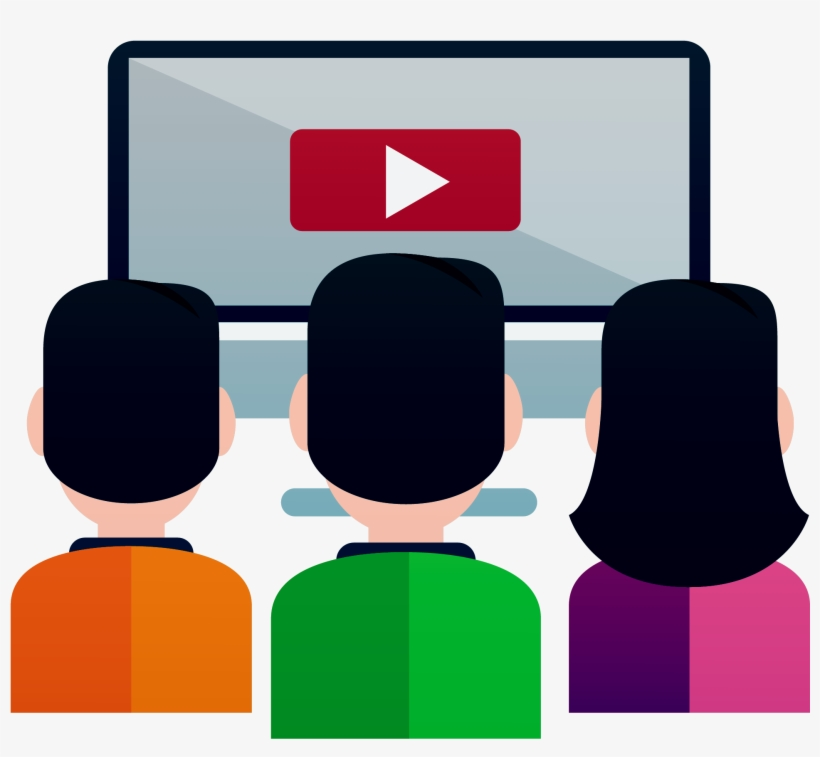
\includegraphics[width=0.55\textwidth]{images/watching_tv.jpeg}
  \end{figure}
\end{frame}

%------------------------------------------------
\section{FLAMeS-Framework}
%------------------------------------------------

\begin{frame}
\frametitle{Analyse realer Netzwerkaktivität}
\begin{itemize}
  \item Datengetriebene Analysen ($30$\textsc{TB} von $300$\textsc{K} Geräten)
  \item Framework FLAMeS\footnote{\textbf{F}ramework for \textbf{L}arge-scale \textbf{A}nalysis of 
  \textbf{M}obil\textbf{e} \textbf{S}ocieties.} zur Analyse
  \begin{figure}
    \centering
    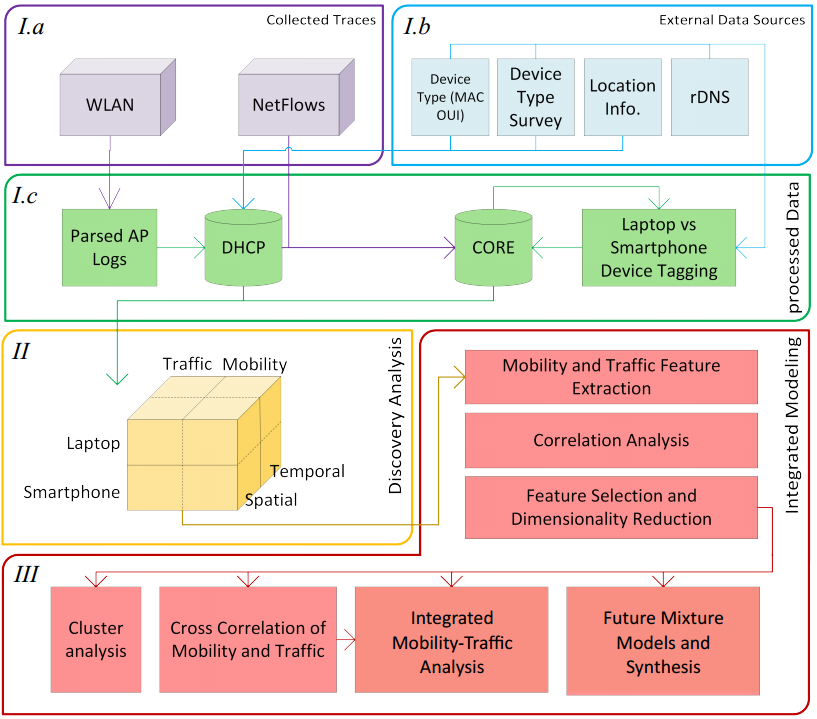
\includegraphics[width=0.6\textwidth]{images/FLAMeS.png}\newline  
  \end{figure}  
\end{itemize}
\end{frame}

%------------------------------------------------
\subsection{\textbf{Phase I}: Datensammlung \& Preprocessing}
%------------------------------------------------

\begin{frame}
  \frametitle{Phase I: Datensammlung \& Preprocessing}

  \begin{figure}
    \centering
    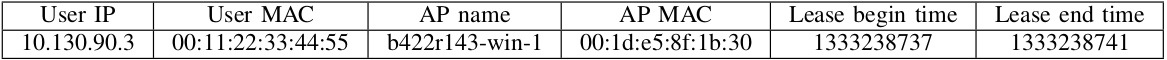
\includegraphics[width=\textwidth]{images/AP_entry.png}
    \caption*{Quelle 1: WLAN-AP-Logs}
  \end{figure}

  \begin{figure}
    \centering
    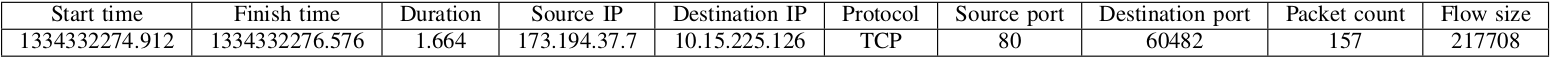
\includegraphics[width=1\textwidth]{images/netflow_entry.png}
    \caption*{Quelle 2: Netflow-Logs}
  \end{figure}
  
  \textbf{Datenbasis}: \textbf{Quelle 1} + \textbf{Quelle 2} (MAC-to-IP-Mapping)
\end{frame}

\begin{frame}
  \frametitle{Phase I: Datensammlung \& Preprocessing}
  \textbf{Heuristik zur Geräteklassifizierung}
  \begin{itemize}
    \item Hersteller mittels OUI identifizieren
    \item Kontakt zu \textit{admob.com} prüfen
  \end{itemize}
  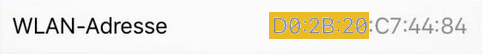
\includegraphics[width=0.8\textwidth]{images/MAC_iPhone.png}\newline
  Wireshark OUI Lookup Tool $\implies$ Apple, Inc.\newline\newline
  Ergebnis: $86\%$ der Geräte in den AP-Logs und $97\%$ der Netflow-Traces klassifiziert
\end{frame}

\begin{frame}
  \frametitle{Phase I: Datensammlung \& Preprocessing}
  \begin{figure}
    \centering
    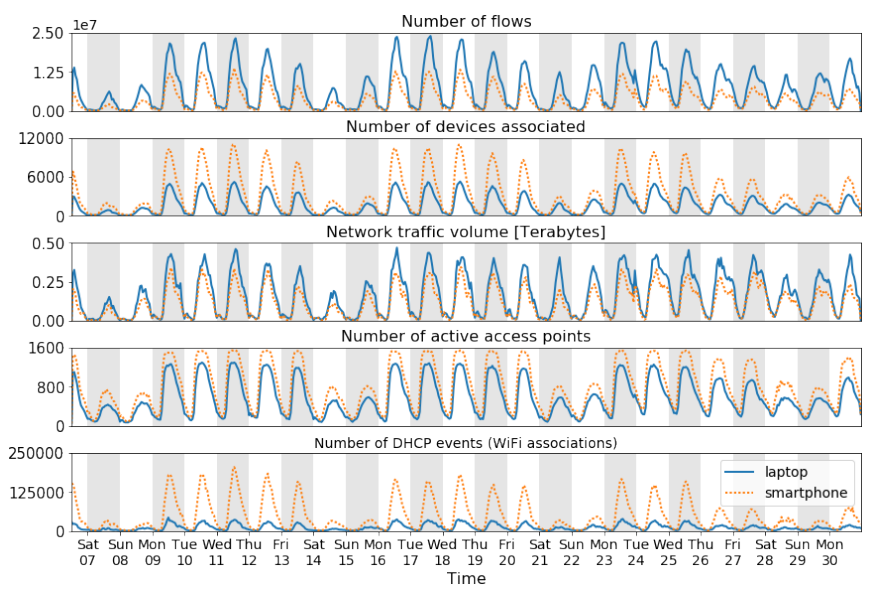
\includegraphics[width=0.8\textwidth]{images/traces.png}
    \caption*{Kombinierte WLAN-AP- und Netflow-Traces}
  \end{figure}  
\end{frame}

%------------------------------------------------
\subsection{\textbf{Phase II}: Analyse der erhobenen Daten}
%------------------------------------------------

\begin{frame}
  \frametitle{Phase II: Zeitliche und räumliche Analyse der Mobilität}
  \begin{itemize}
    \item WLAN-Sessions $\approx$ Startzeiten von Vorlesungen
    \item Aktivität von Laptops fällt nach Ende der Vorlesungszeiten
    \item Abend-Sessions vermehrt in sozialen Einrichtungen / Bib.
    \item Vorlesungen geben Wochentagen Struktur
    \item Substanzielle Reduktion der Mobilität von Laptops
    \item Smartphones \textquote{Always-on-Devices} $\implies$ leichter zu erfassen
    \item Laptops besitzen längere Aufenthaltszeiten 
  \end{itemize}
\end{frame}

\begin{frame}
  \frametitle{Phase II: Zeitliche und räumliche Analyse des Datenverkehrs}
  \begin{itemize}
    \item Smartphone-Flows und Pakete größer
    \item Laptops verursachen $\boldsymbol{\o \thinspace 3.7}$ mal so viele Flows\newline
    \phantom \quad\quad\quad\quad\quad\quad\quad\quad\thinspace\thinspace\thinspace\thinspace\thinspace $\boldsymbol{\o \thinspace 1.6}$ mal mehr Pakete\newline
    \phantom \quad\quad\quad\quad\quad\quad\thinspace\thinspace $\implies \boldsymbol{\o \thinspace 2.7}$ mal so viel Traffic
    \item Wochenenden: Verbleibende Geräte besonders aktiv
    \item Smartphones mehr extreme Phasen der Inaktivität
    \item Laptops ($\boldsymbol{78.5 \%}$ TCP), Smartphones ($\boldsymbol{98.2 \%}$ TCP)
    \item Großteil der APs an Wochenenden nicht verwendet
  \end{itemize}
\end{frame}

\begin{frame}
  \frametitle{Phase II: Zeitliche und räumliche Analyse des Datenverkehrs}

  \begin{figure}[H]
    \centering
    \resizebox{0.6\textwidth}{!}{
    \begin{tabular}{|c|c|c|}
      \cline{1-3}
       & Laptops & Smartphones \\ \cline{1-3}
      AP Volumen (\textbf{\textsc{GB}}) & $\boldsymbol{<5}$ & $\boldsymbol{<3}$ \\ \cline{1-3}
      Datenkonsum (\textbf{\textsc{MB}}) & $\boldsymbol{<700}$ & $\boldsymbol{<200}$ \\ \cline{1-3}
      Aktivitätszeit (\textbf{Std.}) & $\boldsymbol{<3.5}$ & $\boldsymbol{<1}$ \\ \cline{1-3}
    \end{tabular}}
    \end{figure}

    \begin{itemize}
      \item Smartphone-Traffic bursty mit größeren Flows und kleinerer aktiver Dauer
      \item Smartphones insgesamt für deutlich weniger Last verantwortlich
    \end{itemize}
\end{frame}

%------------------------------------------------
\subsection{\textbf{Phase III}: Korrelationen und integrierte Modelle}
%------------------------------------------------

\begin{frame}
  \frametitle{Exkurs: Feature-Engineering}

  \begin{figure}
    \centering
    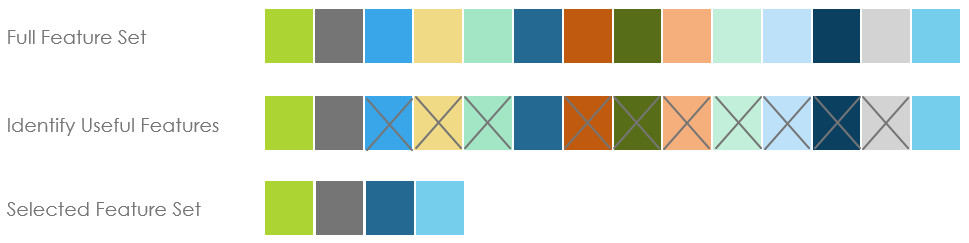
\includegraphics[width=\textwidth]{images/feature_engineering.png}
  \end{figure}

  \begin{itemize}
    \item Correlation Feature Selection (CFS)
    \item \textquote{Person-Correlation}-Methode
  \end{itemize}  
\end{frame}

\begin{frame}
  \frametitle{Phase III: Korrelationen}
  CFS selektiert $5 / 8$ Mobilitäts- und $11 / 19$ Traffic-Features

  \begin{figure}[H]
    \centering
    \begin{subfigure}[b]{0.4\textwidth}
      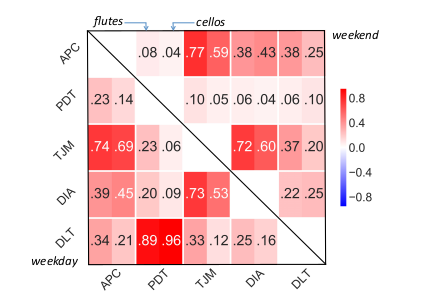
\includegraphics[width=1.2\textwidth]{images/mobility_correlations.png}
      \caption*{Mobilität}
    \end{subfigure}
    \hspace{10px}
    \begin{subfigure}[b]{0.4\textwidth}
      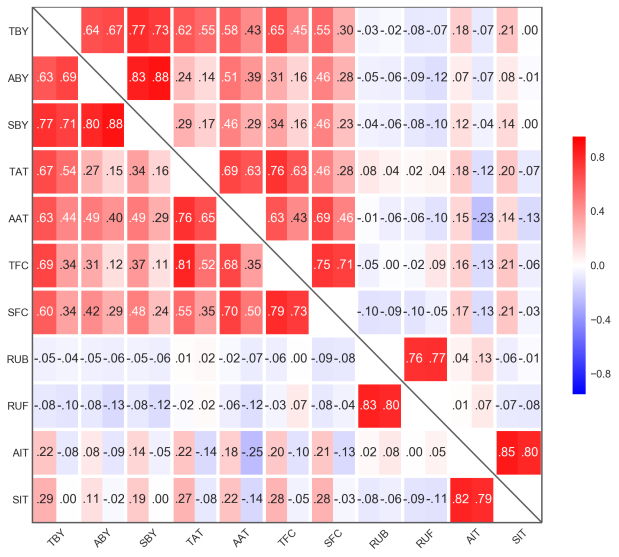
\includegraphics[width=1.2\textwidth]{images/traffic_correlations.png}  
      \caption*{Traffic}
    \end{subfigure}    
  \end{figure}  
\end{frame}

\begin{frame}
  \frametitle{Phase III: Korrelationen zwischen Mobilität und Datenverkehr}
  \begin{figure}
    \centering
    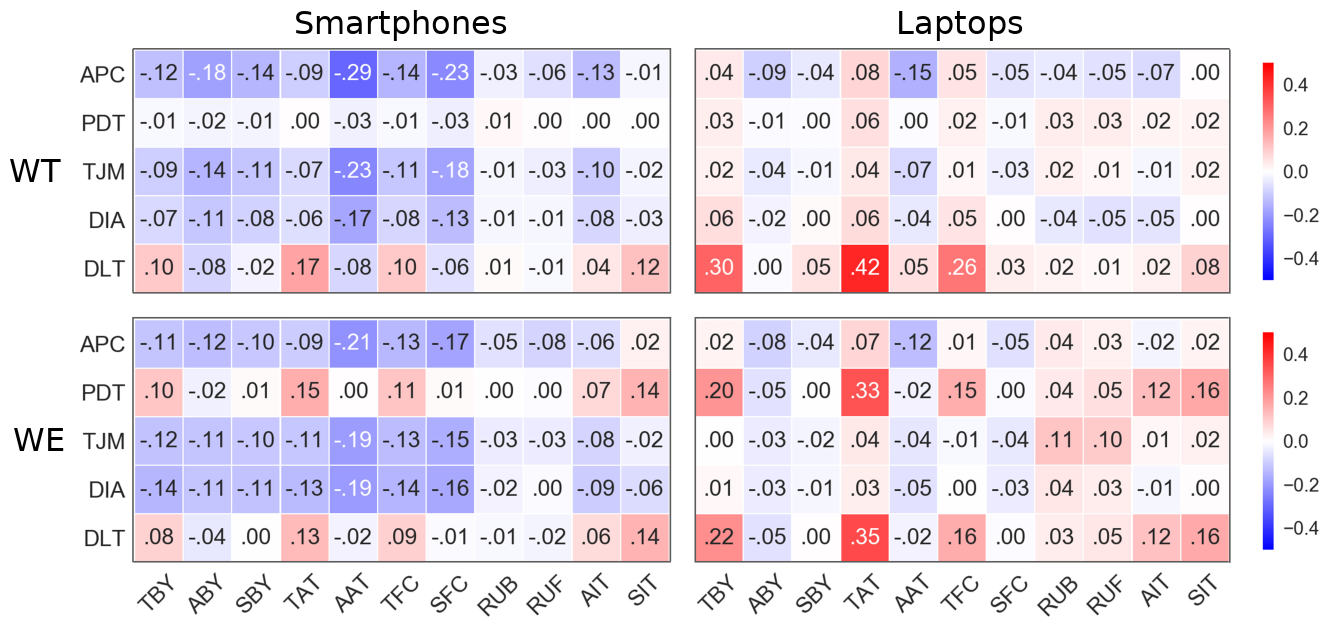
\includegraphics[width=0.8\textwidth]{images/correlations.png}
    \caption*{Korrelationen zwischen Mobilitäts- und Traffic-Features (Wochentage oben, Wochendenden unten,
    Smartphones links, Laptops rechts).}
  \end{figure}
\end{frame}

\begin{frame}
  \frametitle{Phase III: Analyse verschiedener Modelle}
  \textbf{Unterschiede der Mobilitäts- und Traffic-Charakteristiken zwischen den Gerätetypen signifikant?}
  \begin{itemize}
    \item SVM: Kombinierte Modelle mit $\approx 81\%$ genauer als isolierte Modelle (Mobilität $\approx 65 \%$, Datenverkehr $\approx 79 \%$)
    \item Genauigkeit erhöht sich auf $\approx 86\%$, wenn zwischen Wochendenden und Wochentagen differenziert wird    
    \item $k$-Means-Clustering: Kombinierte Features $\approx81.5 \%$ (Mobilität $\approx 60 \%$, Traffic $\approx 81.2 \%$)
  \end{itemize}
\end{frame}

\begin{frame}
  \frametitle{Phase III: Kombiniertes Modell}
  \begin{itemize}
    \item Generierung erster Traces: GMM mit kombinierten Features
    \item Vergleich der generierten Samples mit Echtdaten
    \item Datenverkehr-Features der Samples entsprechen den Originaldaten besser als isoliert trainierte GMM
    \item Keine Verbesserung in Bezug auf die Mobilität
  \end{itemize}
\end{frame}

\begin{frame}
  \frametitle{Zusammenfassung}
  \begin{itemize}
    \item Framework FLAMeS zur Analyse bestehender Traces
    \item Geräteklassifizierung
    \item Untersuchung der Mobilitäts- und Datenverkehrmetriken (Gerätetypen, Zeit, Ort)
    \item Signifikante Unterschiede zwischen den Gerätetypen
    \item Machine Learning --> Kombiniertes Modell --> bildet Unterschiede besser ab als isolierte Modelle
  \end{itemize}  
\end{frame}

%------------------------------------------------
\section{Fazit und Ausblick}
%------------------------------------------------

\begin{frame}
  \frametitle{Weitere Ansätze}
  \textbf{Nutzergruppen}
  \begin{itemize}
    \item Mobilität und Datenverkehr nicht nur zwischen Gerätetypen unterschiedlich
    \item Alter und Geschlecht eines Nutzers berücksichtigen
    \item Kulturellen Kontext aufgezeichneter Daten berücksichtigen    
  \end{itemize}
\end{frame}

\begin{frame}
  \frametitle{Fazit}
  \begin{itemize}
    \item Bisher existierende Modelle nicht detailliert genug
    \item Intuitive Idee eines Zusammenhangs bestätigt
    \item Anstoß für Entwicklung zukünftiger kombinierter Modelle
    \item Konzeption und Validierung eines konkreten Modells wird zukünftiger Forschung überlassen    
  \end{itemize}
\end{frame}

\begin{frame}
  \frametitle{Ausblick}
  \begin{itemize}
    \item Vorhersagbarkeit menschlicher Mobilität
    \item Bewegung von \textquote{sit-to-use}-Geräten besser vorhersagbar
    \item Signifikante Korrelationen zwischen Vorhersagegenauigkeit, Mobilitäts- und Traffic-Features
    \item Untersuchung der Vorhersagegenauigkeit als Feature in integrierten Modellen
    \item Realistische Modellierung der Netzwerkaktivität ist aktives Forschungsfeld
  \end{itemize}  
\end{frame}

\end{document}
